\chapter{Instalación de cliente LDAP en los nodos login-0 y login-1}
Como parte del acondicionamiento del clúster Cadejos y el nuevo diseño de la arquitectura, se requiere de la implementación de dos nodos que administren el inicio de sesión al clúster. Parte de esta implementación implica la instalación y puesta en marcha de los clientes LDAP para su correcto funcionamiento. La implementación anterior con Scientific Linux daba serios problemas de inicio remoto de sesión pues no leía las contraseñas adecuadamente, y únicamente permitía el acceso cuando se habían copiado previamente las llaves SSH. Es por estas razones que se decide migrar la instalación a CentOS 7 puro y se reimplementan los clientes LDAP.  

\section{Montar los directorios en red /home y /opt}
Previo a proceder con la instalación del LDAP es recomendable tener los directorios de interés previamente montados en cada uno de los nodos. El caso particular de /opt es para efectos de poder utilizar los nodos como parte del clúster de memoria distribuida y poder mantener una única instalación de bibliotecas, programas y herramientas, lo cual se cubrirá más adelante. Abrimos el archivo /etc/fstab como root, y agregamos lo siguiente al final:
%%%%%%%%%%%%%%%%%%%%%%%%%%%%%%%%%%%%%%%%%%%%%%%%%%%%%%%%%%%%%%%%%%%
\begin{lstlisting} 
#home
sol3.cnca:/export/ClusterHome            /home   nfs     defaults        0	 0

#opt
sol3.cnca:/export/ClusterOpt            /opt   nfs     defaults        0       0

#scratch
10.0.0.4:/mnt/scratch					/scratch nfs defaults	0	0
\end{lstlisting}
%%%%%%%%%%%%%%%%%%%%%%%%%%%%%%%%%%%%%%%%%%%%%%%%%%%%%%%%%%%%%%%%%%%
Ahora simplemente montamos 
%%%%%%%%%%%%%%%%%%%%%%%%%%%%%%%%%%%%%%%%%%%%%%%%%%%%%%%%%%%%%%%%%%%
\begin{lstlisting} 
mount -a
\end{lstlisting}
%%%%%%%%%%%%%%%%%%%%%%%%%%%%%%%%%%%%%%%%%%%%%%%%%%%%%%%%%%%%%%%%%%%
\section{Instalación de webmin y paquetes LDAP}
Se debe realizar lo siguiente para tener un cliente LDAP funcional:
%%%%%%%%%%%%%%%%%%%%%%%%%%%%%%%%%%%%%%%%%%%%%%%%%%%%%%%%%%%%%%%%%%%
\begin{lstlisting} 
su -
service sshd start
systemctl enable sshd.service
service firewalld stop
systemctl disable firewalld.service
yum remove NetworkManager
yum remove PackageKit
yum update
mkdir software
cd software
wget http://jaist.dl.sourceforge.net/project/webadmin/webmin/1.801/webmin-1.801-1.noarch.rpm
yum -y install perl-LDAP perl perl-Net-SSLeay openssl perl-IO-Tty openssl-devel perl-Crypt-SSLeay
wget https://dl.fedoraproject.org/pub/epel/epel-release-latest-7.noarch.rpm
wget https://rpms.remirepo.net/enterprise/remi-release-7.rpm
rpm --import https://www.elrepo.org/RPM-GPG-KEY-elrepo.org
wget http://www.elrepo.org/elrepo-release-7.0-2.el7.elrepo.noarch.rpm
yum localinstall *.rpm
yum install httpd
systemctl start httpd.service
systemctl enable httpd.service
systemctl start webmin.service
systemctl enable webmin.service
yum remove sssd-client
\end{lstlisting}
%%%%%%%%%%%%%%%%%%%%%%%%%%%%%%%%%%%%%%%%%%%%%%%%%%%%%%%%%%%%%%%%%%%
Una vez realizado lo anterior, procedemos a modificar la configuración de webmin para que no requiera del uso de SSL para su despliegue. Con un editor cualquiera abrimos el archivo /etc/webmin/miniserv.conf y cambiamos la línea ssl=1 por ssl=0. Salvamos y reiniciamos el webmin.
%%%%%%%%%%%%%%%%%%%%%%%%%%%%%%%%%%%%%%%%%%%%%%%%%%%%%%%%%%%%%%%%%%%
\begin{lstlisting} 
systemctl restart httpd.service webmin.service
\end{lstlisting}
%%%%%%%%%%%%%%%%%%%%%%%%%%%%%%%%%%%%%%%%%%%%%%%%%%%%%%%%%%%%%%%%%%%
Ahora procedemos a instalar los paquetes que corresponden al LDAP.
%%%%%%%%%%%%%%%%%%%%%%%%%%%%%%%%%%%%%%%%%%%%%%%%%%%%%%%%%%%%%%%%%%%
\begin{lstlisting} 
yum install openldap openldap-clients nss-pam-ldapd python-ldap lynx authconfig perl-LDAP
systemctl enable nslcd.service
systemctl enable nscd.service
\end{lstlisting}
%%%%%%%%%%%%%%%%%%%%%%%%%%%%%%%%%%%%%%%%%%%%%%%%%%%%%%%%%%%%%%%%%%%
Vamos a utilizar el asistente authconfig-tui para inicializar el cliente LDAP, y posteriormente vamos a realizar modificaciones puntuales en los archivos finales de configuración.
%%%%%%%%%%%%%%%%%%%%%%%%%%%%%%%%%%%%%%%%%%%%%%%%%%%%%%%%%%%%%%%%%%%
\begin{lstlisting} 
authconfig-tui
\end{lstlisting}
%%%%%%%%%%%%%%%%%%%%%%%%%%%%%%%%%%%%%%%%%%%%%%%%%%%%%%%%%%%%%%%%%%%
Nos aparecerá una pantalla como el de la figura \ref{fig:ldapconf:00}, en la cual se muestra el tipo de configuración que se desea realizar. Se le da en aceptar y aparecerá ahora una ventana preguntando por el uso del TLS, cuya casilla dejaremos desmarcada. En la línea de Server escribimos ldap://meta.cnca, y finalmente en la línea de Base DN escribimos dc=cnca,dc=cenat. Aceptamos los ajustes.
%%%%%%%%%%%%%%%%%%%%%%%%%%%%%%%%%%%%%%%%%%%%%%%%%%%%%%%%%%%%%%%%%%%
\begin{figure}[H]
\centering
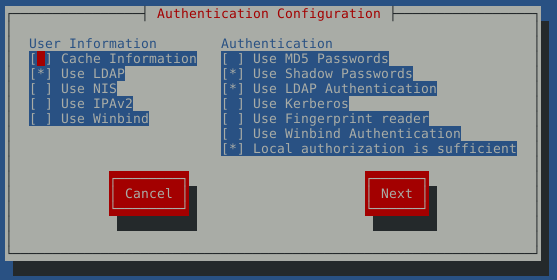
\includegraphics[width=0.45\textwidth]{ldap_conf00.png}
\caption{Pantalla configuración de authconfig-tui.}
\label{fig:ldapconf:00}
\end{figure}
%%%%%%%%%%%%%%%%%%%%%%%%%%%%%%%%%%%%%%%%%%%%%%%%%%%%%%%%%%%%%%%%%%%
Ahora revisamos los archivos /etc/pam.d/password-auth, /etc/pam.d/system-auth, /etc/nsswitch.conf, los cuales deberán verse como se muestra a continuación. Si hay algo que no luce igual, lo recomendable es ajustar para que los archivos sean iguales a como se indican en este documento \cite{ldapserver}.
Para el archivo de configuración /etc/pam.d/password-auth:
%%%%%%%%%%%%%%%%%%%%%%%%%%%%%%%%%%%%%%%%%%%%%%%%%%%%%%%%%%%%%%%%%%%
\begin{lstlisting} 
#%PAM-1.0
# This file is auto-generated.
# User changes will be destroyed the next time authconfig is run.
auth        required      pam_env.so
auth        sufficient    pam_unix.so nullok try_first_pass
auth        requisite     pam_succeed_if.so uid >= 500 quiet_success
auth        sufficient    pam_ldap.so use_first_pass
auth        required      pam_deny.so

account     required      pam_unix.so broken_shadow
account     sufficient    pam_localuser.so
account     sufficient    pam_succeed_if.so uid < 1000 quiet
account     [default=bad success=ok user_unknown=ignore] pam_ldap.so
account     required      pam_permit.so

password    requisite     pam_pwquality.so try_first_pass local_users_only retry=3 authtok_type=
password    sufficient    pam_unix.so sha512 shadow nullok try_first_pass use_authtok
password    sufficient    pam_ldap.so use_authtok
password    required      pam_deny.so

session     optional      pam_keyinit.so revoke
session     required      pam_limits.so
-session     optional      pam_systemd.so
session     [success=1 default=ignore] pam_succeed_if.so service in crond quiet use_uid
session     required      pam_unix.so
session     optional      pam_ldap.so

# autocreate home dirs
session required pam_exec.so /opt/create_scratch.sh
session required pam_mkhomedir.so skel=/etc/skel/ umask=0022
\end{lstlisting}
%%%%%%%%%%%%%%%%%%%%%%%%%%%%%%%%%%%%%%%%%%%%%%%%%%%%%%%%%%%%%%%%%%%
El script create\_scratch.sh automatiza el proceso de creación del directorio para acceder al sistema de archivos no respaldado llamado scratch \cite{pamexec} \cite{pamexec2}. Dicho script se muestra a continuación:

\begin{lstlisting}
#!/bin/bash
mkdir /mnt/scratch/$PAM_USER
chown $PAM_USER:cluster /mnt/scratch/$PAM_USER
ln -s /mnt/scratch/$PAM_USER /home/$PAM_USER/scratch
\end{lstlisting}

Para el archivo de configuración /etc/pam.d/system-auth:
%%%%%%%%%%%%%%%%%%%%%%%%%%%%%%%%%%%%%%%%%%%%%%%%%%%%%%%%%%%%%%%%%%%
\begin{lstlisting} 
#%PAM-1.0
# This file is auto-generated.
# User changes will be destroyed the next time authconfig is run.
auth        required      pam_env.so
auth        sufficient    pam_unix.so nullok try_first_pass
auth        requisite     pam_succeed_if.so uid >= 500 quiet_success
auth        sufficient    pam_ldap.so use_first_pass
auth        required      pam_deny.so

account     required      pam_unix.so broken_shadow
account     sufficient    pam_localuser.so
account     sufficient    pam_succeed_if.so uid < 1000 quiet
account     [default=bad success=ok user_unknown=ignore] pam_ldap.so
account     required      pam_permit.so

password    requisite     pam_pwquality.so try_first_pass local_users_only retry=3 authtok_type=
password    sufficient    pam_unix.so sha512 shadow nullok try_first_pass use_authtok
password    sufficient    pam_ldap.so use_authtok
password    required      pam_deny.so

session     optional      pam_keyinit.so revoke
session     required      pam_limits.so
-session     optional      pam_systemd.so
session     [success=1 default=ignore] pam_succeed_if.so service in crond quiet use_uid
session     required      pam_unix.so
session     optional      pam_ldap.so

# autocreate home dirs
session required pam_mkhomedir.so skel=/etc/skel/ umask=0022
\end{lstlisting}
%%%%%%%%%%%%%%%%%%%%%%%%%%%%%%%%%%%%%%%%%%%%%%%%%%%%%%%%%%%%%%%%%%%
Para el archivo de configuración /etc/nsswitch.conf
%%%%%%%%%%%%%%%%%%%%%%%%%%%%%%%%%%%%%%%%%%%%%%%%%%%%%%%%%%%%%%%%%%%
\begin{lstlisting} 
# /etc/nsswitch.conf
# An example Name Service Switch config file. This file should be
# sorted with the most-used services at the beginning.
#
# The entry '[NOTFOUND=return]' means that the search for an
# entry should stop if the search in the previous entry turned
# up nothing. Note that if the search failed due to some other reason
# (like no NIS server responding) then the search continues with the
# next entry.
# Valid entries include:
#
#	nisplus			Use NIS+ (NIS version 3)
#	nis			Use NIS (NIS version 2), also called YP
#	dns			Use DNS (Domain Name Service)
#	files			Use the local files
#	db			Use the local database (.db) files
#	compat			Use NIS on compat mode
#	hesiod			Use Hesiod for user lookups
#	[NOTFOUND=return]	Stop searching if not found so far
#
# To use db, put the "db" in front of "files" for entries you want to be
# looked up first in the databases
#
# Example:
#passwd:    db files nisplus nis
#shadow:    db files nisplus nis
#group:     db files nisplus nis

passwd:     files ldap
shadow:     files ldap
group:      files ldap
#initgroups: files

#hosts:     db files nisplus nis dns
hosts:      files dns

# Example - obey only what nisplus tells us...
#services:   nisplus [NOTFOUND=return] files
#networks:   nisplus [NOTFOUND=return] files
#protocols:  nisplus [NOTFOUND=return] files
#rpc:        nisplus [NOTFOUND=return] files
#ethers:     nisplus [NOTFOUND=return] files
#netmasks:   nisplus [NOTFOUND=return] files     

bootparams: nisplus [NOTFOUND=return] files

ethers:     files
netmasks:   files
networks:   files
protocols:  files
rpc:        files
services:   files

netgroup:   files ldap

publickey:  nisplus

automount:  files ldap
aliases:    files nisplus
\end{lstlisting}
%%%%%%%%%%%%%%%%%%%%%%%%%%%%%%%%%%%%%%%%%%%%%%%%%%%%%%%%%%%%%%%%%%%
Reiniciamos los servicios correspondientes
%%%%%%%%%%%%%%%%%%%%%%%%%%%%%%%%%%%%%%%%%%%%%%%%%%%%%%%%%%%%%%%%%%%
\begin{lstlisting} 
systemctl restart nslcd.service nscd.service slapd.service
\end{lstlisting}
%%%%%%%%%%%%%%%%%%%%%%%%%%%%%%%%%%%%%%%%%%%%%%%%%%%%%%%%%%%%%%%%%%%
Una vez realizado esto, abrimos una instancia de Firefox en el meta nodo y nos conectamos al webmin recién instalado en el nodo de login  (\url{http://IP_login:10000}). Iniciamos sesión como root, como se muestra en la figura \ref{fig:ldapconf:01}. En la barra de búsqueda a la izquierda escribimos ldap y presionamos enter, como se muestra en la figura \ref{fig:ldapconf:02}. De ahí nos dirigimos al link que dice LDAP Client, como se muestra en la figura \ref{fig:ldapconf:03}. Nos aparece una pantalla como la que se muestra en la figura \ref{fig:ldapconf:04}, en la cual presionamos el botón Start LDAP Client Daemon, y habilitamos el Start LDAP CLient At Boot y luego presionamos el botón Validate Configuration. Luego de esto, nos dirigimos al botón en la barra superior que dice LDAP Browser y aceptamos la instalación del paquete sugerido, en caso de que así lo sugiera, y revisamos que la configuración esté en orden, pues se deben desplegar los grupos y usuarios en la sintaxis de LDAP, como se muestra en la figura \ref{fig:ldapconf:05} \cite{webmininstall}.
%%%%%%%%%%%%%%%%%%%%%%%%%%%%%%%%%%%%%%%%%%%%%%%%%%%%%%%%%%%%%%%%%%%
\begin{figure}[H]
\centering
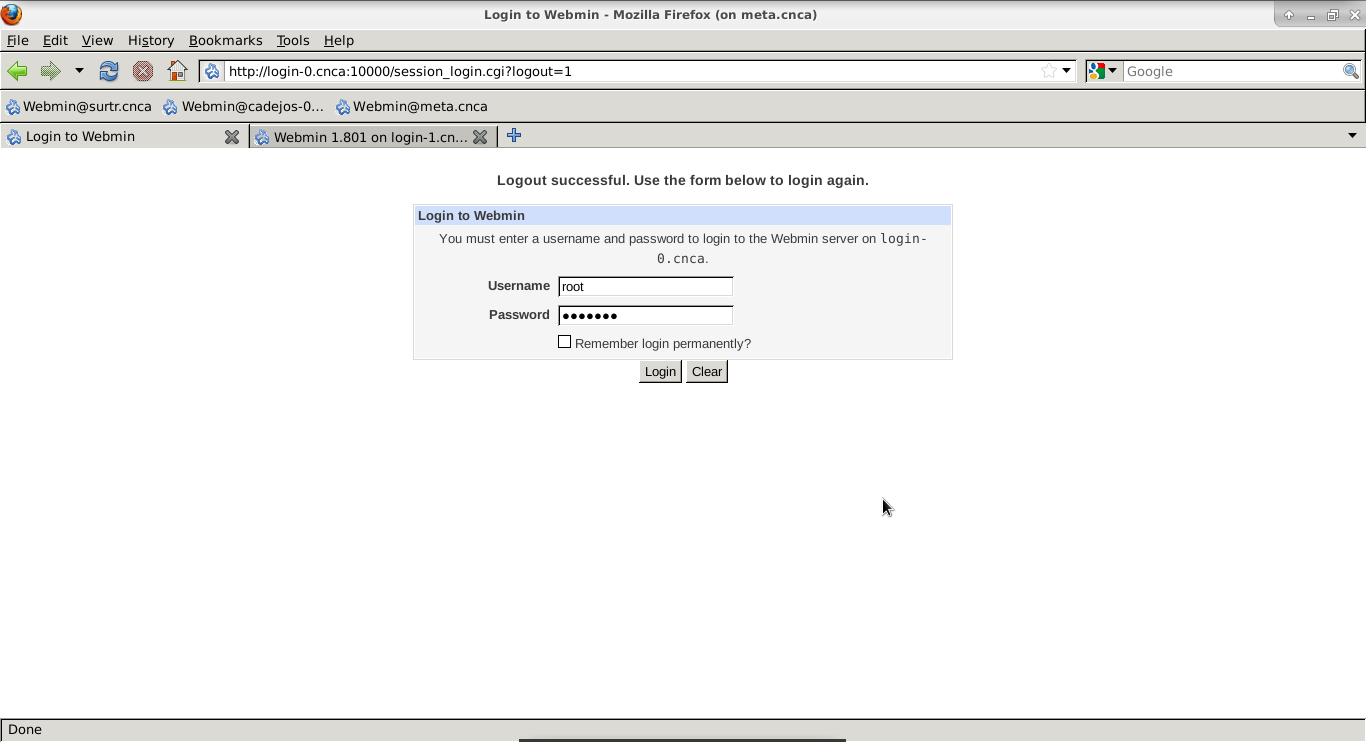
\includegraphics[width=0.45\textwidth]{ldap_conf01.png}
\caption{Inicio de sesión en webmin.}
\label{fig:ldapconf:01}
\end{figure}
%%%%%%%%%%%%%%%%%%%%%%%%%%%%%%%%%%%%%%%%%%%%%%%%%%%%%%%%%%%%%%%%%%%
\begin{figure}[H]
\centering
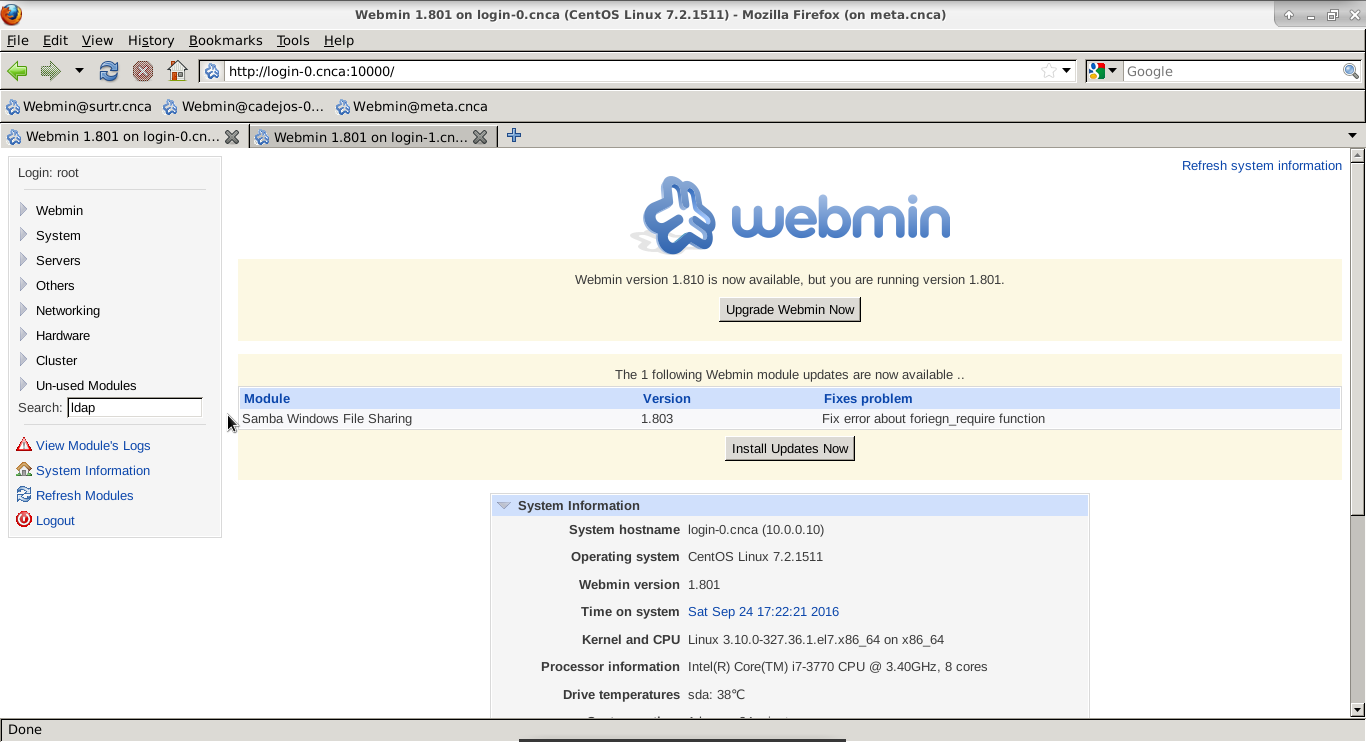
\includegraphics[width=0.45\textwidth]{ldap_conf02.png}
\caption{Búsqueda de componentes del LDAP en webmin.}
\label{fig:ldapconf:02}
\end{figure}
%%%%%%%%%%%%%%%%%%%%%%%%%%%%%%%%%%%%%%%%%%%%%%%%%%%%%%%%%%%%%%%%%%%
\begin{figure}[H]
\centering
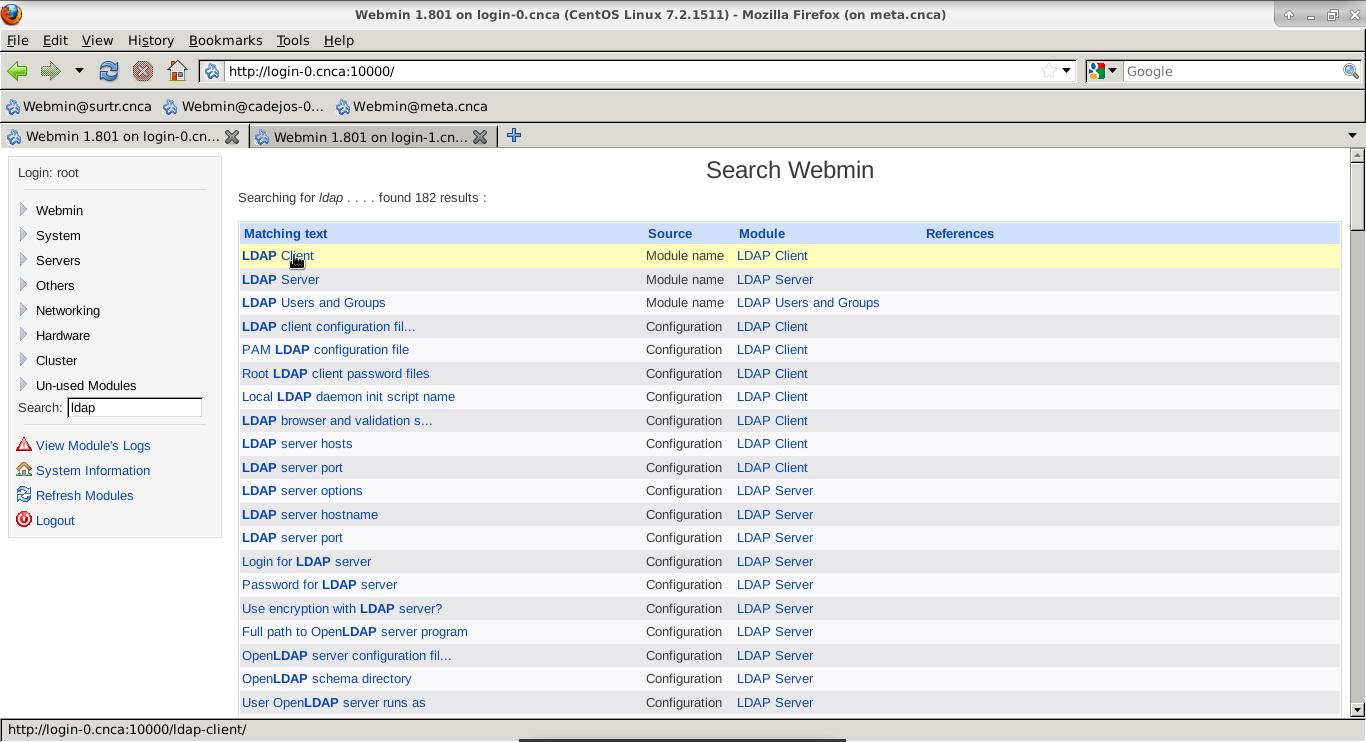
\includegraphics[width=0.45\textwidth]{ldap_conf03.png}
\caption{Ingreso a la ventana de configuración del cliente LDAP en webmin.}
\label{fig:ldapconf:03}
\end{figure}
%%%%%%%%%%%%%%%%%%%%%%%%%%%%%%%%%%%%%%%%%%%%%%%%%%%%%%%%%%%%%%%%%%%
\begin{figure}[H]
\centering
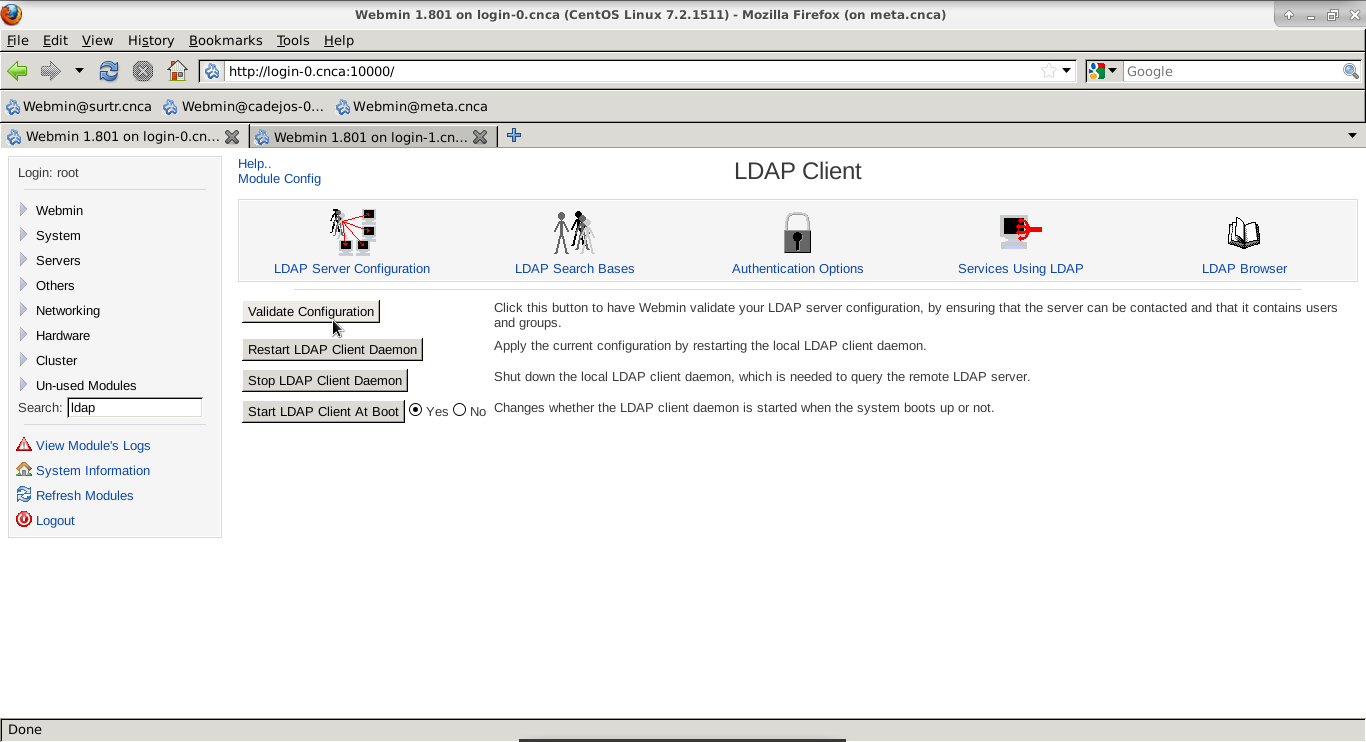
\includegraphics[width=0.45\textwidth]{ldap_conf04.png}
\caption{Ajustes del cliente LDAP en webmin.}
\label{fig:ldapconf:04}
\end{figure}
%%%%%%%%%%%%%%%%%%%%%%%%%%%%%%%%%%%%%%%%%%%%%%%%%%%%%%%%%%%%%%%%%%%
\begin{figure}[H]
\centering
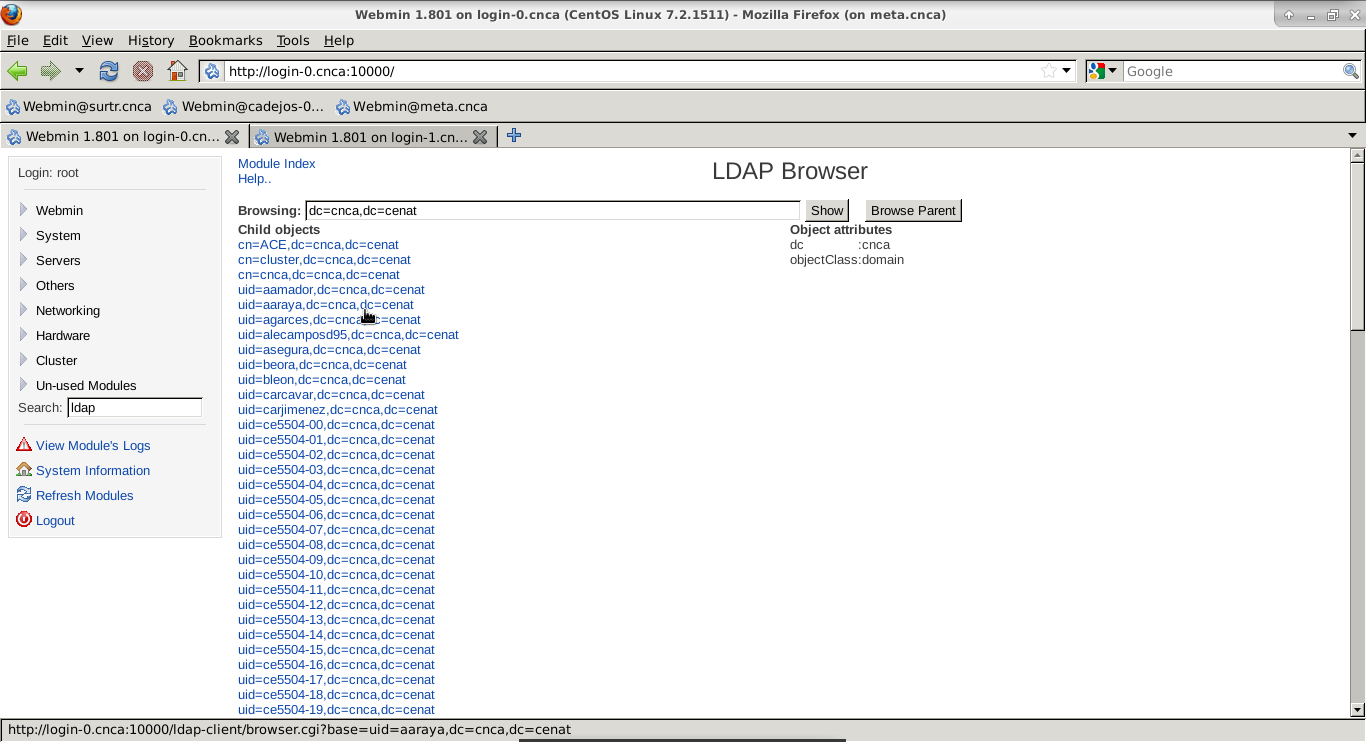
\includegraphics[width=0.45\textwidth]{ldap_conf05.png}
\caption{Información visible tras la configuración del cliente LDAP en webmin.}
\label{fig:ldapconf:05}
\end{figure}
%%%%%%%%%%%%%%%%%%%%%%%%%%%%%%%%%%%%%%%%%%%%%%%%%%%%%%%%%%%%%%%%%%%
\section{Conflicto al cambiar la contraseña por primera vez}
A algunos usuarios se les ha presentado problemas para cambiar la contraseña de su cuenta, mostrando el siguiente error:
%%%%%%%%%%%%%%%%%%%%%%%%%%%%%%%%%%%%%%%%%%%%%%%%%%%%%%%%%%%%%%%%%%%
\begin{lstlisting}
Changing password for user su-usuario
(current) LDAP Password: 
New password: 
Retype new password: 
password change failed: Insufficient access
passwd: Authentication token manipulation error
\end{lstlisting}
%%%%%%%%%%%%%%%%%%%%%%%%%%%%%%%%%%%%%%%%%%%%%%%%%%%%%%%%%%%%%%%%%%%
Para resolver este conflicto, accedemos al meta nodo y editamos el archivo 
/etc/openldap/slapd.d.org/cn=config/olcDatabase={2}bdb.ldif y agregamos lo siguiente al final \cite{passwdldap}.
%%%%%%%%%%%%%%%%%%%%%%%%%%%%%%%%%%%%%%%%%%%%%%%%%%%%%%%%%%%%%%%%%%%
\begin{lstlisting}
###### Agregado	por problemas con cambio de contraseña
olcAccess: {0}to attrs=userPassword by self write by dn.base="cn=Manager,dc=cnca,dc=cenat" write by anonymous auth by * none
olcAccess: {1}to * by dn.base="cn=Manager,dc=cnca,dc=cenat" write by self write by * read
\end{lstlisting}
%%%%%%%%%%%%%%%%%%%%%%%%%%%%%%%%%%%%%%%%%%%%%%%%%%%%%%%%%%%%%%%%%%%
Con esto debería resolverse satisfactoriamente el conflicto.
\clearpage